\documentclass[ngerman]{tudscrreprt}

\usepackage{babel}
\usepackage[utf8]{inputenc}
\usepackage{todonotes}


\newcommand{\todogrf}{\todo{add graphic here}}
\newcommand{\todosct}{\todo{add section here}}
\newcommand{\todoedit}{\todo{edit this section}}

\begin{document}
	\faculty{Faculty Computer Science}
	\institute{Institute of Systems Architecture}
	\chair{Chair of Computer Networks}
	\date{15.11.2019}
	\author{Sinthujan Thanabalasingam}
	\title{Redesign and unification of the web view of AMCS}
	\maketitle
	
\begin{abstract}
	
Auditorium Mobile Classroom Service (AMCS) is an Audience Response system that is actively developed by several individuals at the TU Dresden since 2012. In the educational context, speakers and docents use it to enhance and manage their lectures during the semester. One of the main goals of AMCS is to improve the way knowledge is presented and transferred to the audience by offering interactive polls that students can participate in before, during and after a lecture.
Several standalone front end applications for platforms like iOS, Android and web are provided that enable usage of the system. However because of its ease of access, a majority of students use the system via their web browsers on different mobile devices such as laptops, tablets and smartphones. 
Regarding usability, design and consistency, the challenge lays in providing a unified and responsive user interface across all supported platforms that is intuitive to use. DUDE
	
\end{abstract}


\chapter{Introduction}

\section{Motivation}


AMCS (Auditorium Mobile Classroom Service) is an Audience Response System (ARS) currently under development at the TU Dresden. Several members of the Faculty of Computer Science initialized the project in 2012 and since then, the system and its community have grown continuously and countless features were added over the years.
\newline
\newline
In general, the system's main objective is to improve the way knowledge is transferred from a speaker to their audience. By providing interactive polls and evaluation mechanisms, AMCS aims at increasing the audience's engagement before, during and after a lecture takes place, overall strengthening the interaction between speaker and audience.
\newline
\newline
On the one hand, several features of AMCS are designed to support speakers in their role. Regarding the educational context, lecturers at university use it not only during their lecture to get immediate feedback from participating students. Furthermore, it is used during the whole semester to prepare and manage lectures, to analyze learning progress and to evaluate feedback given by students. More specifically, a speaker can gain insight on the understanding of their audience by evaluating answers to their polls. For example, poor results to a poll covering a certain topic might suggest that the topic was misunderstood or badly explained. AMCS enables the speaker to precisely use  this information, helping to identify parts of their lectures that students might struggle with. Speakers can focus more easily on repeating and emphasizing these topics in the future.
\newline
\newline
On the other hand, AMCS provides a set of features that try to increase engagement and to close the gap between speaker and listener.
One of the system's goals is to support a student's learning process by providing interactive polls, question pools and self-evaluation mechanisms that work on saved answers. While the polls are often used during lectures, the latter two tools can be used afterwards to identify and repeat difficult questions, to prepare for the next lesson or to study for the examination. 
\newline
\newline
Several standalone front end applications for different platforms such as iOS, Android and web are provided to the audience. However AMCS is used by the majority of students via its web page across different mobile devices such as laptops, tablets and smartphones, likely because it is very easy to access.
\newline
\newline 
Regarding the web page being the most common way AMCS is used, 
the challenge lays in providing a unified and responsive web-based user interface across all aforementioned device types. The motivation of this work is to analyze the application's state in terms of usability, design and consistency, identify weaknesses in each category and provide a set of proposals that hope to improve the design currently in place.

\section{Objective}
\label{section:intro:objective}
The main objective of this work is to provide a redesign strategy that - when implemented - improves the web view of AMCS on mobile devices in order to create a more user friendly experience. AMCS does offer a variety of features to the audience and to speakers. They were designed and developed by different people over the years and therefore all differ  variously in terms of UI design and layout.
To keep the scope of this work manageable, this work will mostly focus on all features that audience members will come in contact with when using AMCS.
Each proposal for itself is centered around improving usability of the application while all proposals as a whole aim at keeping a consistent and recognizable interface across all supported platforms.  Therefore, the rest of this work is structured as follows:
\newline
\newline
Chapter \ref{chapter:stateoftheart} describes the current state of the application and briefly covers all features of AMCS that fall in the redesign strategy scope.
Additionally, in section \ref{section:soa:related}, relevant existing applications and work are analyzed to identify strategies that can be transferred and applied to AMCS.
\newline
\newline
Following up is chapter \ref{chapter:concept} that is divided in two main sections. In section \ref{section:con:problems}, an analysis of the current state of the application is conducted, identifying weaknesses and inconsistencies that the design can be improved on.
In Section \ref{section:con:proposals} these weaknesses are subject of discussion in a redesign strategy that is described in detail.
\newline
\newline
Finally, in chapter \ref{chapter:implementation} the redesign strategy it is implemented as a prototype that uses the existing back end system.
Chapter \ref{chapter:evaluation} evaluates the prototype and compares it to the current state of AMCS.
\newline
\newline
Chapter \ref{chapter:conclusion} concludes this work by giving a short outlook on future work.

\chapter{Current State of AMCS}
\label{chapter:stateoftheart}
At the time of writing, AMCS provides front end applications for iOS, Android and web that students can use. AMCS does offer a variety of features to the audience and to speakers. They were designed and developed by different people over the years and therefore all differ variously in terms of UI design and layout.
To keep the scope of this work manageable, this work will mostly focus on all features that audience members will come in contact with when using AMCS.
This section elaborates on the current state of the system by identifying and analyzing all views that allow for access to the different functionalities of AMCS from a student's point of view. 

\section{Web Technologies}
The AMCS front end web page is written using Angular\footnote{https://angular.io (\emph{last access: 01.11.2019})}, a typescript-based front end framework for building mobile and desktop web applications.

\section{Landing Page and Login}
\label{section:landingpage}
When accessing the website\footnote{https://amcs.website (\emph{last access: 01.11.2019})}, students will be shown the landing page of AMCS (see \Cref{fig:landingpage}). A big login button is displayed that when pressed will reveal a login form (see \Cref{fig:loginform}).
In order to use the system, students have to create an account by providing credentials.
\newline
\newline
Additionally, a subscription to courses is mandatory in order to reasonably use the service. By typing in an optional PIN code, students will subscribe automatically to the corresponding course. From thereon, students have access to the system. 
 
\begin{figure}
	\centering
	\begin{minipage}[t]{.5\textwidth}
		\centering
 		\includegraphics[width=0.95\linewidth]{screenshots/landing_page.jpg}
		\captionsetup{width=.8\linewidth}
		\caption{The landing page of AMCS. This is the initial screen shown when accessing \emph{https://amcs.website}}
		\label{fig:landingpage}
	\end{minipage}%
	\begin{minipage}[t]{.5\textwidth}
		\centering
		\includegraphics[width=0.95\linewidth]{screenshots/login_form.jpg}
		\captionsetup{width=.8\linewidth}
		\caption{The login form of AMCS. Users can choose a synonym and a password to create an account.}
		\label{fig:loginform}
	\end{minipage}
\end{figure}
 
\section{Main View}
\label{section:soa:mainview}
After successfully logging in, the user is presented with the Main View of the system (see \Cref{fig:mainview}).
It can be scrolled in the vertical direction and is divided into header and body. On top, the header consists of corporate branding on the left side and a burger menu on the right side. Below it, the view's body organizes information in different sections as follows:

\begin{figure}
	\centering
	\begin{minipage}[t]{.5\textwidth}
		\centering
		\includegraphics[width=0.95\linewidth]{screenshots/main_view_1.jpg}
		\captionsetup{width=.8\linewidth}
		\caption{Main View: Lecture information is provided in different sections for each temporal context. Per default, a section with proposed lectures is expanded.}
		\label{fig:mainview}
	\end{minipage}%
	\begin{minipage}[t]{.5\textwidth}
		\centering
		\includegraphics[width=0.95\linewidth]{screenshots/main_view_course_management.jpg}
		\captionsetup{width=.8\linewidth}
		\caption{Course management below Lectures: Each course is listed below an enrollment form consisting of a PIN input and a submit button.}
		\label{fig:mainviewcoursemanagement}
	\end{minipage}
\end{figure}

\subsection{Lectures}
\label{section:soa:mainview:lectures}
This section lists all lectures that the user subscribed to (see \Cref{fig:mainview}). It is organized in subsections that indicate the temporal context of each lecture. These include:

\paragraph{Proposed lectures} - Lectures that the system proposes to the user. These lectures either will take place in the next 24 hours or already occurred in the last 24 hours.
\paragraph{Upcoming lectures} - Lectures that will take place in the future are shown here.
\paragraph{Active lectures} - Lectures that take place right now are shown here.
\paragraph{Past lectures} - Lectures that have already taken place are shown here.

\paragraph{Rendering of lectures}

Each of the aforementioned subsections is organized in a list that contains all corresponding lectures. For each lecture, a box is rendered that uses all horizontal space available to it. The box consists of a blue header with the lecture's name, a white info/detail area and a light blue footer that contains the course name.
A color-coded badge on the top right of the boxes serves as an indicator for the temporal context of the lecture.
The subsections can be collapsed or expanded by clicking on the sections heading.

\todo{add graphic of badges}


\subsection{Course management}

Further down on the page, the section \emph{Enrolled Courses} can be found (see \Cref{fig:mainviewcoursemanagement}). It serves two purposes: Primarily, it provides a way to enroll into a course. An enrollment form is shown that consists of a text field to enter the course PIN and a blue button to trigger the enrollment. When provided with a valid PIN, pressing the button redirects the user to the \emph{Course View} (described in \Cref{section:soa:courseview}) on successful enrollment.
Secondly, the view shows all courses the student is currently enrolled in. They are rendered as light blue buttons in a vertical list. A trash can icon on each button provides a way to leave the given course.

\section{Poll View}
\label{section:soa:pollview}
Answering polls is one of the main functionalities of the system that users will engage with.
Polls can be reached by clicking on a lecture box from either the \emph{Main View} or the \emph{Course View}.
Each poll consists of a set of questions the user can answer. They are rendered in a view that is reused by the system depending on the situation and context. This means that the view might only be accessible under certain circumstances, for example when the lecture reaches a specific point in time, making it a slide poll (SP). SPs are shown when a specific slide is on display and can only be answered in this very moment. Other types of polls include “global” course polls (CP) that are always accessible during the semester and lecture polls (LP) which can only be answered during the life time of a lecture.
Active polls are displayed all at once in sections designated to each poll type.
The different types of polls that occur in AMCS are further summarized in \Cref{tab:pollTypes}.



\begin{table}[H]
	{\renewcommand{\arraystretch}{2}
		\begin{tabular}{ | p{5cm} | p{10cm} |}
			\hline
			Poll Type & Explanation \\ \hline \hline
			Slide Poll (SP) & Active when a specific slide is shown. Commonly used for quizzes after a difficult section in a lecture to make sure that students understood everything correctly. \\ \hline
			Preparation Poll (PP) & Active before the lecture takes place. Is commonly used to instruct students to prepare for a certain topic. \\ \hline
			Lecture Poll (LP) & Active during the lifetime of a lecture. \\ \hline
			Post Processing Poll (PPP) & Active after a lecture has taken place. Commonly used to check gained knowledge. \\ \hline
			Course Poll (CP) & Active during the whole lifetime of the course (commonly during the whole semester). \\
			\hline
		\end{tabular}
	}
	\caption{Different poll types that the user might encounter when using AMCS.}
	\label{tab:pollTypes}
\end{table}

If no polls for a given lecture are available, the user is presented with the hint shown in \todogrf.

\section{Course View}
\label{section:soa:courseview}

The \emph{Course View} is shown when the user selects one of the courses from the course management section (see \Cref{fig:courseview} and \Cref{fig:courseviewlectures}). Its purpose is essentially to provide a filtered view on the lectures of a single course.
The course name and PIN, it's description and lists of upcoming, live and past lectures are visible from top to bottom in this order. It reuses the lecture section component described in \Cref{section:soa:mainview:lectures}.

\begin{figure}
	\centering
	\begin{minipage}[t]{.5\textwidth}
		\centering
		\includegraphics[width=0.95\linewidth]{screenshots/course_view_1.jpg}
		\captionsetup{width=.8\linewidth}
		\caption{\emph{Course View}: Details like the course name, description and PIN are displayed.}
		\label{fig:courseview}
	\end{minipage}%
	\begin{minipage}[t]{.5\textwidth}
		\centering
		\includegraphics[width=0.95\linewidth]{screenshots/course_view_3.jpg}
		\captionsetup{width=.8\linewidth}
		\caption{Lectures that belong to a certain course displayed in the \emph{Course View}.}
		\label{fig:courseviewlectures}
	\end{minipage}
\end{figure}


\section{Menu and Navigation}
Besides using the \emph{Main View}, additional functionality can be reached by navigating the burger menu that is shown in the upper-right corner of the screen. It reveals a sub menu which expands vertically, offering three additional sub menus (see Figure \todosct). In the following, these sub menus and their functionality are briefly explained.

\subsection{Student}

This is one of the most important buttons that connects a subset of main functionalities of AMCS. Upon pressing this button, the menu expands again vertically, showing a list of further sub menus. Most of the functionalities shown in this list will be touched by the proposals for improvement that are presented in \Cref{chapter:concept}. The functionalities in questions are:

\begin{enumerate}
	\item Evaluation of answers
	\item Question Pool
	\item Edit account
\end{enumerate}

\subsubsection{Evaluation of Answers}

Once students have participated in a poll and answered a few questions, they can evaluate their answers by selecting this option. Two drop down menus are shown prompting the student to select the course and lecture they are interested in. 
After choosing an item from the list, a vertical list of all questions that occurred during this lecture is shown to the student, together with indicators for the given answers.
If the student used two attempts to answer the question, a toggle button is provided to switch between the first and the second answer. \todogrf

\subsubsection{Question Pool}

By selecting this option from the \emph{Burger Menu}, the student is offered the possibility to create collections of already answered questions. The intent is to provide a way for students to collect and repeat questions that they had difficulty in answering.
Similar to \todosct, the student is prompted with a drop down menu to select a course they are interested in. After selection, the student is presented with a list of all lectures and their polls respectively. All questions of each poll are grouped and shown to the student in a vertical list. From this list, the student can select all questions that they might be interested in to create a pool of questions.
These pools are composed into polls that the student then can answer again. These polls are rendered in the same manner as stated in \Cref{section:soa:pollview}.


\subsubsection{How It Works}

Pressing this button will redirect to a page that shows tutorial instructions on how to use AMCS.
This help page is rendered identical on all mobile devices and therefore falls out of the scope of this paper.

\subsubsection{Logout}

As the name already states, pressing this button will logout the user and end the session. 
If logging out was successful, the \emph{Landing Page} is displayed.




\begin{figure}
	\centering
	\begin{minipage}[t]{.5\textwidth}
		\centering
		\includegraphics[width=0.95\linewidth]{screenshots/expanded_burger_menu.jpg}
		\captionsetup{width=.8\linewidth}
		\caption{Expanded \emph{Burger Menu}.}
		\label{fig:menu}
	\end{minipage}%
	\begin{minipage}[t]{.5\textwidth}
		\centering
		\includegraphics[width=0.95\linewidth]{screenshots/course_view_3.jpg}
		\captionsetup{width=.8\linewidth}
		\caption{Lectures that belong to a certain course displayed in the \emph{Course View}.}
		\label{fig:other}
	\end{minipage}
\end{figure}

\section{Summary}
The identified UI components that will be further analyzed and discussed are summarized in the following table:

\begin{table}[H]
	{\renewcommand{\arraystretch}{2}
		\begin{tabular}{ | p{4cm} | p{11cm} |}
			\hline
			Component & Description \\ \hline \hline
			Landing Page & Shown when the web page is opened. Points to the Login mechanism. \\ \hline
			Main View & Gives an overview of ongoing lectures and enrolled courses. Allows to enroll to or unsubscribe from courses. \\ \hline
			Poll View & Shown whenever a poll should be answered. \\ \hline
			Course View & Displays information and lectures of a single course. \\ \hline
			Burger Menu & Overarching navigation element visible in all views. \\ \hline
			Question Pool & Shown when the creation of a question pool is attempted. Can be reached from the \emph{Burger Menu}. \\ \hline
			Evaluation of answers & Shown when the evaluation of answers to polls is attempted. Can be reached from the \emph{Burger Menu}. \\ \hline
		\end{tabular}
	}
	\caption{Summary of UI Components discussed in this work.}
	\label{tab:components}
\end{table}


\chapter{Concept}
This chapter will cover identified problems that occur when using AMCS via a web browser on mobile
devices. To narrow down the extend of this work, the system is analyzed from the point of view that an audience member like a student has while using AMCS on their smartphone. When doing so, students will interact mostly with the Main View and the Navigation, which are the components that this work will focus on.

\section{Problems of the mobile view}

The web page of AMCS reacts on requests coming from mobile devices such as smartphones or tablets by providing a responsive mobile view to its clients. However, in some aspects AMCS struggles to offer a UI experience that guarantees high usability and uniformity across all end user devices.
One challenge lays in the fact that the system has to deal with limited screen space to visualize information as effectively as possible. Additionally, users might approach the application with different ways of interaction and navigation in mind that are typical for mobile devices. For example, a smartphone user might expect to be able to use swiping gestures to navigate a menu or that information is organized in views consisting of separate tabs. This section lists key issues that lower usability or might cause confusion to users when using the system on a smartphone.

\subsection{Main View}
As already described in section \todosct, the main view relies on a vertically scrolling list view, consisting of different sections. The layout in place causes problems regarding usability aspects of the application.

\subsubsection{General Visualization Problems}
\label{section:con:problems:mainview:generalvis}
Section \todosct covered the fact, that lectures are rendered by displaying the title of the lecture in the top section of the box in white letters on a solid blue background. It is followed by detail information about the lecture such as time, duration and a textual description, visualized in gray letters and icons in a white screen. Finally, at the bottom of the box, the course name is shown in gray letters on a light blue background. The order "lecture name then details and then course name" can cause confusion to students.

The most coarse grain piece of information - the course name - is displayed at the bottom of the box rather than at the top. Generally, when seeking information about active lectures, a student will most likely remember the course name rather than the name of a single lecture, as timetables used by students only contain course names. Therefore, displaying the course information in this order might cause confusion and students take longer time to find the pieces of information that they are looking for.
In addition to that, background colors and font size are used to differentiate between course name and lecture name, further supporting the ambiguity described above.

\subsubsection{Indirection Problems}

The boxes that represent each lecture claim a lot of screen space in relation to the information that is displayed to the student. The layout causes a lot of indirection, because per default, the sections for upcoming and active lectures are expanded fully. This might be handy when quickly gathering information about lectures that are or soon will be active, but in every other case it slows navigation and overall interaction, because the course management section is pushed down to the bottom of the page.
A list of only four boxes causes a scroll bar to appear on the very common screen resolution of 1920x1080 pixels. A student that navigates to the main view to enroll into a new course therefore always has to scroll to the bottom of the page before they reach the enrollment form. The same problem likewise occurs when simply seeking information about what courses a student is already enrolled in or when trying to leave a course altogether. 

Further more, if a student looks for information regarding a specific course, no filter or search functionality is offered by the lecture list. Instead, they have to scroll down to the bottom of the lecture list, scan the course list manually with their eyeballs, find the course and click on the corresponding item. Finally, they are redirected to the course view. This level of indirection is only further increased the more courses the student is enrolled in. 
To sum it up, the hierarchical and logical relationship between courses and lectures is broken. 

\subsubsection{Redundancy}

Some visual redundancy is added by the badges that are displayed on the top right corner of each lecture. These badges are used to visualize the temporal context of the lecture for each item in the corresponding section. It seems that the badge's intention is to help conveying the temporal context of the lecture, because sorting the lectures in their respective section alone fails to do so. Furthermore, the badge's names do not match the section's names, e.g. an upcoming lecture's badge reads “BEFORE” instead of “UPCOMING”. 

In the course management section below, for each course the student is enrolled in, a box is shown with the course's name along with an unsubscribe button, represented by a trash can icon.
\todogrf
This is a redundant way of rendering the courses which adds noise to the overall look of the view and uses much of the vertical screen estate.

\subsection{Course View}

Since the course view reuses the lecture list along with the sections “Upcoming lectures”, “Active lectures” and “Past lectures”, likewise the same issues arise as for the main view, as already described in section \ref{section:con:problems:mainview:generalvis}. 
The course view has a very important function in terms of usability as it acts as a filter for lectures belonging to a certain course. Problems arise, when a user wants to switch quickly between different courses. Doing so requires to leave the course view by tapping the back button and then scanning the course management section for the element of interest, which is slow and cumbersome.

\todogrf

\subsection{Poll View}

\subsubsection{Rendering}

Section \todosct describes the rendering of questions as boxes that are aligned in a vertical scrolling list. This introduces similar problems as already described in section 3.1, namely the extensive use of vertical space on the screen. Bigger polls that consist of multiple questions unnecessarily take a lot of vertical screen estate. The view also lacks of basic information such as number of questions in total or number of remaining questions that might be useful in bigger polls if students want to gain an overview of how many questions are left.
Answering one question usually does not require to see the neighboring questions, but most of the time, two to three questions are in view simultaneously. This might be distracting to some students.
\todo{Provide screenshots and explain this better.}
Additionally, the layout lacks of separation and distinction between types of polls.
Different types of polls are simply appended to the bottom of the list, making it even longer.

\subsubsection{Local navigation}

The vertical list is difficult to navigate as it requires scrolling between questions. If a student wants to jump from the first to the last question,  or vice versa, several swiping gestures are needed to reach the top or the bottom of the list.
Similar to the lecture list described in \todosct, the question list is also segmented into different sections. Lecture and course questions are similarly appended to the bottom of a slide poll. This means again, that a student that wants to view these questions has to scroll all the way to the bottom of the list. Again, this layout introduces a lot of indirection and is not intuitive to the user.


\subsection{Burger Menu and Navigation}

At the time of writing, the ways of navigating the application can be described as problematic and partly confusing. Several layers of indirection introduce problems and may worsen the user experience.
Figure \ref{figure:clickpathproblems} illustrates that the click paths a user must take in order to reach different views (illustrated in blue) within AMCS. In general, some views are connected via the burger menu as the overarching element of navigation (illustrated in green). In contrast, other views are interconnected and can be reached by clicking on elements inside a view such as a course or lecture. The following paragraphs elaborate more on both aspects of navigation.

On the one hand, the interconnected graph of views as it is described in Figure \ref{figure:clickpathproblems} contains two main issues. One example of unexpected behavior is the fact that when a user wants to return from the Poll View to the Main View in order to chose a different poll, they are first redirected to the Course View. However, it is possible to reach the Poll View from the Main View with one tap, by selecting a lecture for example. Furthermore, some views like the Question Pool View and the Answer Evaluation View do not offer buttons that allow to navigate back. The navigation relies partly on the corporate branding on the top left that when tapped will redirect to the Main View.
This means that the interconnectedness between different views might not be strong enough.

On the other hand, the burger menu connects several aspects and functionalities of AMCS in an overarching manner, as it is part of every view. Students have to tap on the icon to access menu that consists of sub menus as described in \todosct. 
One visual problem that arises is the fact that the menu uses a lot of vertical screen space and delocates the rest of the content that is currently shown when several sub menus are expanded. An example as to why this is problematic might be the following scenario: a student wants to evaluate their answers to polls for a certain lecture. When opening the menus on their phone from the Main View, information like course name and lecture title are pushed down by the menu. But this information is required in the Answer Evaluation View because the user is asked to chose their course and lecture of interest from two drop down menus. This could lead to users having to return to the Main View to look up the lecture name or other details again.
In addition to that, the menu can confuse students because the first menu entry is labeled as \emph{Student}. This implies to users in general that there exist different roles that a user can take on in AMCS, which is the case. However the user's role should not be the label of a sub menu in the navigation as it is not intuitive that functionality like account management, the Question Pool and Answer Evaluation can be accessed via a button labeled \emph{Student}.

\subsubsection{Evaluation of answers}

Clicking on the option “Evaluation of answers” button in the expanded burger menu leads to a view with a drop down menu from which students can choose a course that they are interested in. Afterwards, an list of expandable items is shown, where each item represents a lecture. Clicking on one or multiple of these items will expand a vertical list of questions similar to  the regular question list described in section \todosct, but answers given by the student are shown as well (see Fig. \todosct).
Multiple problems occur on this view: First of all, the navigation path to reach this view contains unnecessary indirection and might not be intuitive enough, which is again illustrated by Figure \ref{figure:clickpathproblems}. Students might expect this functionality to be located at the Main View attached to the elements of the course list or inside the Course View itself. Instead, every time evaluation of given answers is attempted, this functionality can only be accessed by using the burger menu, choosing the appropriate item from the sub menu, selecting the course in question and afterwards expand the lecture and the corresponding question list.
Additionally, the question list suffers from the same rendering and navigation problems already described in \todosct. Questions are poorly navigable and a lot of scrolling is needed to jump between questions.



\begin{figure}[ht]
	\centering
	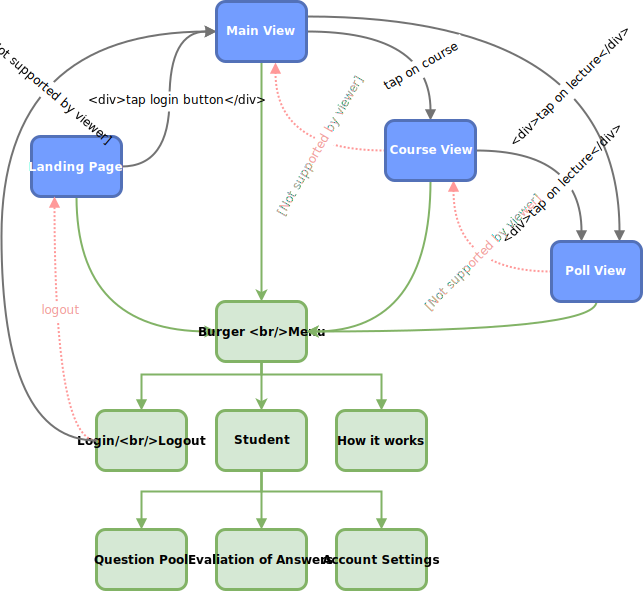
\includegraphics[width=\textwidth]{diagrams/amcs-click-paths.png}
	\caption{Navigation concept of AMCS: Every arrow represents a tap / click the user has to do to reach the desired destination.}
	\label{figure:clickpathproblems}
\end{figure}
\subsubsection{Question Pool}

The question pool suffers from the same navigation problems described in the previous section. Again, a drop down menu for selecting a course is shown before students can see the overview of the question pool. Once more, students might think that access to this functionality is located near the main view or the course view, which is not the case.

\todo{Add a table that names and describes all analyzed weaknesses so that the proposals chapter can refer to this}


\begin{table}[t]
	{\renewcommand{\arraystretch}{2}
		\begin{tabular}{ | p{1cm} | p{2.5cm} |  p{2.5cm} |  p{6cm} |}
			\hline
			ID & Name & Category & Summary \\ \hline \hline
			Slide Poll (SP) & Test & Test & test \\ \hline
		\end{tabular}
	}
	\caption{Different poll types that the user might encounter when using AMCS.}
	\label{tab:problems}
\end{table}


\section{Proposals for Improvement}

Several weaknesses and flaws of the web view of AMCS have been identified and analyzed in the previous section.
The following section introduces a set of proposals that aim at solving these issues. Mainly, the concept will focus on using the available screen space more efficiently, improving local navigation inside polls and global navigation between different screens and views as well as reducing indirection as much as possible.

\subsection{Main View}

\subsubsection{Layout}
As mentioned in section \todosct, the main view suffers from using the vertical space available inefficiently. Most noticeably, the course overview and enrollment form are placed below the list of lectures. In order to find information about relevant courses or to enroll / leave a course, students are required to scroll all the way to the bottom. 
Therefore, one proposal is to compress this view by using drop down menus and tabs (see Fig. 5). First of all, the view is restructured to follow the hierarchical concept of courses containing lectures: In the top (1), a button for a drop down menu is shown next to the currently selected courses name and two additional buttons (6) and (7). The functionality of the drop down menu and the buttons is explained later.
Following the heading, selectable tabs for “past”, “upcoming” and “live” lectures are shown side by side (2). The tab bar is followed by a numbered horizontal list of clickable dots (3) that each represent one lecture. The currently selected lecture is highlighted with a bold blue border to enhance visibility and orientation. Finally, the information section of the view follows (4) with the title of the lecture, time and duration details and the lecture description. In the details view, an additional button is placed (5) that is labeled as “Evaluate”. This button is only available on past lectures, as shown in Figure 5.

This layout reduces the amount of vertical space that is used. The placement of the “Evaluate” button (5) is motivated by reducing vertically occupied space as much as possible, but it could be reasonable to place it below the description text of the lecture. On most devices, the amount of scrolling required should be reduced with the proposed layout. As much redundancy as possible is eliminated from the view, as the badges that indicate temporal context of the lectures now miss completely.

\subsubsection{Navigation}
Tabs (2) should separate lectures by their temporal context. Selecting a tab will display only lectures that share the respective temporal context, meaning that it should be easier to switch between past, upcoming and live lectures.
The “button bar” (3) in Figure 5 is used to ease navigation between lectures that share the same temporal context. A student can use the bar for example to switch quickly between the oldest and newest past lecture by selecting the corresponding button from the bar. This should improve navigation within the main view as well as within a lecture context. 
Additionally, this proposal aims at removing indirection as much as possible on a global scale by providing certain buttons that serve as shortcuts for the functionality that is currently found in the burger menu. Button (6) serves as a shortcut to the Question Pool for the selected course. On click of button (7), the student will be removed from the selected course. Both of these buttons are placed in the header of the layout next to the course’s name to indicate that both referenced functionalities operate on a course scale, whereas the “Evaluate” button (5) operates on a lecture scale. The “Evaluate” button eliminates the need to select a course from a drop down menu and even choosing from a list of lectures is not necessary anymore, as all of these information needed to send the request to the backend are present. Therefore, multiple layers of indirection are removed from the typical workflow. All three buttons try to remove the indirection introduced by the burger menu as much as possible. Functionality that is associated with a course or lecture is triggered from a view that deals with courses and lectures. The burger menu would then only have to deal with the profile editing functionality and the logout functionality.

\subsubsection{Embedded Drop down menu}
The drop down menu (see \todogrf) is introduced to help reducing usage of vertical space even more. Clicking on it reveals its two functions: for one, the enrollment form is now embedded in the drop down menu - a text field and a button are shown next to the text “Enroll...”. The close proximity to courses the student already enrolled into makes this functionality potentially more intuitive to be found by users. The enrollment form will only be embedded in the drop down menu when the student is enrolled in at least one course beforehand. Otherwise, in place of the main view, only the enrollment form should be shown. Besides the enrollment form, a list of courses a student is already enrolled to is shown below. Selecting an item from this list will bring up the corresponding course view, similar to Figure 5. An idea to further enhance the drop down menu would be to show notifications in little bubbles beside the course title to indicate new or upcoming lectures.


\subsection{Poll View}

\subsubsection{Layout}
Several issues have been identified regarding the layout and visualization of polls in section \todosct. Main problems include the ineffective use of vertical space in this view and a lack of separation between types of polls. Different types of polls are simply appended to the bottom of the list, making it even longer. In order to solve these issues, some proposals that were made in \todosct can be applied here as well.  Figure \todosct shows an instance of a slide poll showing a SCC-question using a concept that is proposed in this section.
\todo{Rewrite the sentence above. Its bad}
Beginning at the top, the course's name is displayed in white font on a blue rectangle (1). Following up, to separate the type of polls from one another, a tab based menu is used (2) that differentiates between slide polls, lecture polls and course polls. Each tab therefore corresponds to a poll type. Selecting one of the tabs will cause the layout to show only questions of said type. This will improve the effectiveness of vertical space used greatly. The tabs act as a filter to what is currently displayed.

A further enhancement would be to show notifications in little bubbles besides the name of a tab to indicate new content.
\todo{Find a reference in real life to justify this statement}
 Below the tab menu, a navigation bar (3) is displayed that contains the name of the current topic and additional information such as the number of the current question. In case of a slide poll as shown in Figure 7, the current slide number is shown as well.
Also, the dot bar of section 3.2.1 is reused here (4). The dot bar serves as a means to navigate between questions more easily and faster but also reduces vertical space used significantly. It uses color coding and icons to convey information to the student. A blue bold border is used to indicate the current question selected in the dot bar, light blue dots signify, that the corresponding question has not been answered yet, where as bold green  or red dots indicate correct and wrongly answered questions respectively. The dot bar can be further enhanced by using icons that represent the state of a specific question. Green arrows and red crosses can be used to visualize correctly or wrongly answered questions respectively to ease usability for colorblind students. Below the dot bar, only one question at a time is displayed to the student to avoid overwhelming them (5). The question is displayed in a blue rectangle with white text. Below the question, an instance of an answering mechanism is displayed (6). In the case of SC-, MC-, SCC- or MCC-question, the button to answer the question is omitted. Multiple ideas for triggering the request to the AMCS backend exist here: Either selecting the answer will trigger a modal that asks the user whether or not he is sure with his choice of answer, and confirming this dialog will send the data to the server, or the mere selection of an answer will trigger the request.  A wrong answer is highlighted as before in red, a correct answer in green and it will still be possible to answer twice. Finally, space for textual feedback is given in a box (7) below the answers. This view is reusable and can therefore can also be used to display already answered questions when using the “Evaluate answers” functionality. This view then will also profit from the reduced amount of vertical space used. 

\subsubsection{Navigation between questions}

Navigation between questions should be made easier for students and focus on one question at a time. Therefore, an improvement would be to introduce two buttons in the navigation bar that can be used to navigate one question forward or backwards. Pressing the respective button will cause to show the next or previous question, regardless of whether the current question has already been answered. This leads to the same level of freedom when navigating polls that the current state of the application allows.

Swiping is a widely spread way of interacting with a user interface on smartphones or tablets. Consequently, a student might find it intuitive to use these gestures while using AMCS. Navigating between questions should be possible by swiping left to go forward or right to go backwards. The combination of swiping and the provision of buttons to navigate in the navigation bar helps not to break uniformity between different platforms. This will result in the fact that students on smartphones and tablets have buttons and swipe gestures available to them, while users on laptops and PCs without touchscreens can use the buttons.
In addition to that, the student can use the dot bar to freely select a question they wish to answer or review. This eases navigation within a poll, no scrolling is required anymore.


\subsection{Course View}
\todo{Write about how the course view is eliminated}
\subsection{Navigation}
\todo{Write about how the naviagtion and the burger menu was slimmed}

\todo{Add a table that names and describes all proposals so that the implementation chapter can refer to this}
\chapter{Implementation}
\label{chapter:implementation}

The previous chapter elaborated on a redesign strategy addressing all of the identified issues that impair the usability of AMCS on mobile devices.
This chapter covers the realization of said changes in the form of a prototypical application. However, not all proposals were implemented as specified. One reason for this is that several problems arose during development such as legacy code that could not be changed easily without requiring a complete rewrite. The existing code base is complicated and hard to understand, as several different individuals worked on it over the years. Another reason are some of the proposals themselves, as they were not thought through to the end or even deemed impractical without necessary improvements. Nevertheless, parts of the concept were adapted and a prototype was successfully implemented.
In the following, the implementation process and the required adjustments to the concept will be elaborated by describing different design iterations and the decisions behind each change.

\begin{figure}
	\centering
	\begin{minipage}[t]{.5\textwidth}
		\centering
		\includegraphics[width=0.95\linewidth]{screenshots/redesign/drop_down_student.jpg}
		\captionsetup{width=.8\linewidth}
		\caption{Expanded \emph{Burger Menu}.}
		\label{fig:drop_down_student}
	\end{minipage}%
	\begin{minipage}[t]{.5\textwidth}
		\centering
		\includegraphics[width=0.95\linewidth]{screenshots/redesign/drop_down_lecturer.jpg}
		\captionsetup{width=.8\linewidth}
		\caption{Lectures that belong to a certain course displayed in the \emph{Course View}.}
		\label{fig:drop_down_lecturer}
	\end{minipage}
\end{figure}

\section{Main View}

The \emph{Main View} has undergone several revisions and does not exactly resemble the mock-ups that were shown in the previous chapter (see \Cref{figure:mainviewenhancement3}). The general layout stayed roughly the same, keeping the idea of a \emph{Drop Down Menu} and \emph{Lecture Tabs} below. But a lack of consideration for the different \emph{Roles} users can play when using AMCS made a small number of changes and considerations necessary.
\\

The view consists of the \emph{Drop Down Menu} on the top that allows for course selection and \emph{Lecture Tabs} on the bottom that displays lectures sorted by their temporal context. Between the two of them, a context-sensitive \emph{Actions Menu} is displayed.


\subsection{Drop Down Menu}
Generally speaking, the \emph{Drop Down Menu} provides a coarse grain filter that allows the user to select a specific course. Doing so causes the \emph{Lecture Tabs} and their content to change accordingly.
More specifically, the \emph{Drop Down Menu} acts in a slightly different manner depending on the current user role. When using it as a \emph{Student} (see \Cref{fig:drop_down_student}), it contains all courses that said student is enrolled to. On top of that, the \emph{Enrollment Form} is embedded inside the menu, allowing the \emph{Student} to join other courses.
\\
In contrast, when logged in as a \emph{Lecturer} (see \Cref{fig:drop_down_lecturer}), the \emph{Drop Down Menu} contains all courses that he owns and manages. Naturally, the \emph{Enrollment Form} is omitted as the \emph{Lecturer} role does not need it.
\\
\\
Selecting a course from the list causes an additional component to be displayed: the \emph{Actions Menu}.
\subsection{Actions Menu}
An oversight not covered by the proposals is the fact that the functionality offered by the \emph{Main View} has to change depending on the role of the user that is currently logged in. To address this issue more effectively, the \emph{Actions Menu} is introduced.
The \emph{Actions Menu} offers several buttons with different functionality derived from user roles and privileges.
The number and kind of buttons displayed in the \emph{Actions Menu} varies depending on role of the user that is currently logged in. \emph{Students} are shown the buttons for either visiting the \emph{Question Pool} or \emph{Leaving} the course altogether. In contrast, if a \emph{Lecturer} is logged in, the \emph{Action Menu} contains more options. A \emph{Lecturer} can \emph{Create a Lecture}, \emph{Edit, Export, Clone, Evaluate } or \emph{Delete} a course. Visualization and placement of the \emph{Actions Menu} is explained in the sections following.


\subsection{Lecture Tabs}
Lastly, the \emph{Lecture Tabs} are displayed at the bottom. Each temporal context is associated with a color, label and icon to allow for easier differentiation between them. Similar to the \emph{Actions Menu}, the concept for displaying lectures had to be adapted to comply with the semantics of different user roles.
If a \emph{Student} is logged in, the tabs \emph{Live}, \emph{Upcoming} and \emph{Past} are shown. An additional tab labeled \emph{Offline} is displayed when logged in as a \emph{Lecturer}, as \emph{Lecturers} are able to create lectures in advance and restrict access to them by changing their status to \emph{Offline}.
\\
\\
For each tab, an indicator for the number of lectures belonging to it is provided.
Tapping on one of the tabs displays the lectures in a vertical list. Instead of using paging to divide the content in shorter lists as proposed in \Cref{figure:mainviewenhancement3}, the whole list of lectures is displayed at once.
This decision was made partly because the existing code base was difficult to adapt to these criteria.

\begin{wrapfigure}{r}{0.5\textwidth}
	\vspace*{-2cm}
	\begin{center}
		\includegraphics[width=0.48\textwidth]{screenshots/redesign/main_view_iteration_1.jpg}
	\end{center}
	\caption{Iteration 1 of the \emph{Main View}.}
	\label{fig:main_view:_it1}
	\vspace*{-1.5cm}
\end{wrapfigure}

\subsection{Lecture List}
The visualization of lectures underwent several different iterations before it was finalized for the evaluation. Each iteration introduced small but significant changes to the overall look and feel of the user interface.
In general, each lecture is displayed in a box colored according to the temporal context of the lecture.
The course name is displayed in a smaller font. Below that, the full title of the lecture is shown in a slightly bigger and bold font. Reading this information from top to bottom conveys the hierarchical structure of courses consisting of lectures. 

\subsubsection{Iteration 1}
Lectures are grouped by date and a visual divider between dates is introduced to emphasize and visualize this grouping (see \Cref{fig:main_view:_it1}). Each lecture is displayed in a color coded box. On the top, the date of the lecture is displayed along with two buttons. The first button on the left will redirect to the \emph{Evaluation of Answers} functionality. 
At first, in order to save space, only the course name and the lecture title are shown. The description of the lecture below is deemed not as important and is therefore retracted per default. The second button on the top right can be used to unveil the lecture description.
The \emph{Actions Menu} as such was not part of this iteration yet.

\paragraph{Problems}
The date divider does not eliminate the redundancy introduced by displaying the date of each lecture individually.
Furthermore, the design of the two buttons on the top right might be problematic. For once, it can be difficult to identify these two elements with their placement and lack of textual label as pressable buttons. While collecting intermediate feedback from the AMCS group, people tended to say that they struggle with identifying the meaning of the iconography used. 

\subsubsection{Iteration 2}
The second iteration addresses the problems described above partly (see \Cref{fig:main_view:_it2}). Most notably, the \emph{Lecture List} resembles more a calendar or a student schedule in its overall design. The layout is divided into two columns: The left column displays the current date, whereas the right column contains the list of courses associated to the date. Essentially, instead of displaying the date for each lecture, this information is extracted to the left column. Now, only the time and duration is displayed at the top for each lecture separately.
\begin{wrapfigure}{l}{0.5\textwidth}
	\vspace*{-0.5cm}
	\begin{center}
		\includegraphics[width=0.48\textwidth]{screenshots/redesign/main_view_iteration_2.jpg}
	\end{center}
	\caption{Iteration 2 of the \emph{Main View}. Four tabs are displayed when logged in as a \emph{Lecturer}. From left to right: \emph{Live, Upcoming, Past, Offline}.}
	\label{fig:main_view:_it2}
	\vspace*{-1.5cm}
\end{wrapfigure}
The description remains retractable. The buttons on the top of each lecture have the colors of their background and icon inverted, but they essentially remained the same.
Furthermore, each lecture box is given a drop shadow to indicate that the area is pressable. Pressing anywhere on this \emph{card-like} box will redirect students to the \emph{Poll View}, whereas lecturers will arrive at the \emph{Course Dashboard}.

\paragraph{Problems}
Besides the ambiguity of the buttons at the top of each lecture, each \emph{tab} is suffering from the same problem. According to feedback from the AMCS group, the used iconography alone fails to convey which temporal context each tab is representing.

\subsubsection{Iteration 3}
Some issues regarding the \emph{Lecture List} are fixed in this iteration.
To clarify the meaning of each \emph{tab}, a textual label is added. 
The colors of each tab are adjusted slightly to be more easy on the eyes. Time and duration of each lecture is displayed in one line next to each other. The two buttons previously discussed are moved to the bottom. They are expanded to take most of the width of the lecture box. The icons remain the same but they are reduced in size and pushed to the left.
A textual label in the center of each button now describes its purpose.

This iteration also includes the introduction of the aforementioned \emph{Actions Menu}. It consists of a vertical list of buttons and remains completely hidden if the entry \emph{All courses} is selected from the \emph{Drop Down Menu}. This design hopes to remove unnecessary clutter by displaying these buttons only when needed.

\begin{figure}
	\centering
	\begin{minipage}[t]{.5\textwidth}
		\centering
		\includegraphics[width=0.95\linewidth]{screenshots/redesign/lecture_tab_labels.jpg}
		\captionsetup{width=.8\linewidth}
		\caption{Improved \emph{Lecture Tabs} of \emph{Iteration 3} with textual labels. Either three or four tabs are displayed depending on the user role.}
		\label{fig:main_view_tab_labels}
	\end{minipage}%
	\begin{minipage}[t]{.5\textwidth}
		\centering
		\includegraphics[width=0.95\linewidth]{screenshots/redesign/main_view_it3_lecture_box.jpg}
		\captionsetup{width=.8\linewidth}
		\caption{Improved \emph{Lecture Box} of \emph{Iteration 3}. The two buttons, previously at the top and unlabeled, are now located at the bottom.}
		\label{fig:main_view_lecture_box_buttons}
	\end{minipage}
\end{figure}
\paragraph{Problems}
The introduction of the \emph{Actions Menu} raises new problems. The buttons are organized in a vertical list that pushes all following content further down the page. This problem is essentially identical to the issue that occurred with the original \emph{Burger Menu}. After pressing one of the buttons of the \emph{Actions Menu}, content below might change. However, in some cases, because the menu itself stays in place, these updates of the user interface below might happen completely off screen. Therefore, selecting some of the buttons could feel to the user like an idempotent operation.
\begin{figure}
	\vspace*{-1cm}
	\centering
	\begin{minipage}[t]{.5\textwidth}
		\centering
		\includegraphics[width=0.95\linewidth]{screenshots/redesign/problem_main_view_course_actions.jpg}
		\captionsetup{width=.8\linewidth}
		\caption{\emph{Actions Menu for Lecturer} in \emph{Iteration 3}: The \emph{Lecture Tabs} are displaced by the long list of buttons. }
		\label{fig:main_view_course_options_bad}
	\end{minipage}%
	\begin{minipage}[t]{.5\textwidth}
		\centering
		\includegraphics[width=0.95\linewidth]{screenshots/redesign/main_view_iteration_4_actions.jpg}
		\captionsetup{width=.8\linewidth}
		\caption{Improved \emph{Actions Menu} of \emph{Iteration 4}: An extra button donated by three dots (in the red square) opens an overlay that contains the \emph{Actions Menu}.}
		\label{fig:main_view_course_options_good}
	\end{minipage}
\end{figure}



\subsection{Iteration 4}
\begin{wrapfigure}{r}{0.5\textwidth}
	\vspace*{-0.5cm}
	\begin{center}
		\includegraphics[width=0.48\textwidth]{screenshots/redesign/main_view_iteration_4.jpg}
	\end{center}
	\caption{\emph{Iteration 4}: The \emph{Action Menu} now is accessed by pressing the \emph{Three-Dots-Button} next to the \emph{Drop Down Menu}. An indicator for unanswered polls is added to the \emph{Lecture Box}.}
	\label{fig:main_view_iteration_4}
\end{wrapfigure}
\emph{Iteration 4} represents the last incremental update to the \emph{Main View}.
Most prominently, the  \emph{Action Menu} is now hidden per default. 
A new button next to the \emph{Drop Down Menu} suggests additional options that concern the selected course. Tapping this button shows the \emph{Action Menu} (see \Cref{fig:main_view_course_options_good}). Selecting one of the options from the \emph{Actions Menu} causes it to close and update the view below accordingly.
Furthermore, changes to the \emph{Lecture Tabs} are made. The \emph{Notification Bubbles} are changed slightly in style. They now serve as absolute counter for the number of elements inside a tab.
Besides this change, a \emph{Notification Bubble} is displayed for each \emph{Lecture Box}, indicating new and unanswered questions for a given lecture.
\\
\\ 
\section{Navigation}
As proposed earlier in \Cref{chapter:concept}, the \emph{Burger Menu} was slimmed down considerably. A logged in user can only find the menu entries \emph{Profile}
, \emph{How it works} and \emph{Logout}.
The \emph{Question Pool} and \emph{Evaluation of Answers} is moved to the respective lectures in the \emph{Main View}. Apart from these changes, the \emph{Burger Menu} stayed the same.



\section{Poll View}


\subsection{Navigation between Questions}

\include{evaluation}
\include{conclusion}

\appendix
\section{Appendix Title}

This is the text of the appendix, if you need one.


% We recommend abbrvnat bibliography style.

\bibliographystyle{abbrvnat}

% The bibliography should be embedded for final submission.

\begin{thebibliography}{}
	
	\bibitem[Smith et~al.(2009)Smith, Jones]{smith02}
	P. Q. Smith, and X. Y. Jones. ...reference text...
	
\end{thebibliography}

\end{document}